%%%%%%%%%%%%%%%%%%%%%%%%%%%%%%%%%%%%%%%% IMPORTS %%%%%%%%%%%%%%%%%%%%%%%%%%%%%%%%%%%%%%%%
\documentclass[11pt,onesize,a4paper,titlepage]{article}

%%%%%%%%%%%%%%% Formatting %%%%%%%%%%%%%%% 
\usepackage[english]{babel}
\usepackage[utf8]{inputenc}
\usepackage{geometry} % Margins
\usepackage{sectsty} % Custom Sections

%%%%%%%%%%%%%%% Font %%%%%%%%%%%%%%% 
\usepackage{Archivo}
\usepackage[T1]{fontenc}

%%%%%%%%%%%%%%% Graphics %%%%%%%%%%%%%%% 
\usepackage{fontawesome5} % Icons
\usepackage{graphicx} % Images
\usepackage[most]{tcolorbox} % Color Box
\usepackage{xcolor} % Colors
\usepackage{tikz} % For Drawing Shapes
\tcbuselibrary{breakable}

%%%%%%%%%%%%%%% Miscelanous %%%%%%%%%%%%%%% 
\usepackage{lipsum} % Lorem Ipsum
\usepackage{hyperref} % For Hyperlinks

%%%%%%%%%%%%%%% Colors %%%%%%%%%%%%%%% 
\definecolor{title}{HTML}{5D8AA8} % Color of the title
\definecolor{backdrop}{HTML}{5D8AA8} % Color of the side column
\definecolor{lightgray}{HTML}{b8b8b8} % Color for the skill bars

%%%%%%%%%%%%%%% Section Format %%%%%%%%%%%%%%% 
\sectionfont{                     
    \LARGE % Font size
    \sectionrule{0pt}{0pt}{-8pt}{1pt} % Rule under Section name
}

\subsectionfont{
    \large % Font size
    \fontfamily{phv}\selectfont % Font family
    \sectionrule{0pt}{0pt}{-8pt}{1pt} % Rule under Subsection name
}

%%%%%%%%%%%%%%% Margins and Headers %%%%%%%%%%%%%%%
\geometry{
  a4paper,
  left=7mm,
  right=7mm,
  bottom=10mm,
  top=10mm
}

\pagestyle{empty} % Empty Headers
%%%%%%%%%%%%%%%%%%%%%%%%%%%%%%%%%%%%%%%% MACROS %%%%%%%%%%%%%%%%%%%%%%%%%%%%%%%%%%%%%%%%

%%%%%%%%%%%%%%% Link With an Icon %%%%%%%%%%%%%%% 
\newcommand{\link}[1]{
    \href{#1}{\faIcon{link}}
}

%%%%%%%%%%%%%%% Name Template %%%%%%%%%%%%%%% 
\newcommand{\name}[2]{
    % Name
    \Huge % Font size
    \raggedright \textbf{#1} \par

    \vspace*{0.3cm}
    
    % Profession
    \Large % Font size
    \raggedright #2 \par
    \normalsize \normalfont
}

%%%%%%%%%%%%%%% Contact Details %%%%%%%%%%%%%%%
\newcommand{\info}[2]{
    \faIcon{#2} \hspace{0.2em} #1
}

%%%%%%%%%%%%%%% Email %%%%%%%%%%%%%%%
\newcommand{\email}[1]{
    \info{#1}{envelope}
}

%%%%%%%%%%%%%%% Phone Number %%%%%%%%%%%%%%%
\newcommand{\phone}[1]{
    \info{#1}{mobile-alt}
}

%%%%%%%%%%%%%%% Address %%%%%%%%%%%%%%%
\newcommand{\address}[1]{
    \info{#1}{map-marker-alt}
}

%%%%%%%%%%%%%%% GitHub %%%%%%%%%%%%%%%
\newcommand{\github}[2]{
    \info{\href{#1}{\underline{#2}}}{github}
}

%%%%%%%%%%%%%%% LinkedIn %%%%%%%%%%%%%%%
\newcommand{\linkedin}[2]{
    \info{\href{#1}{\underline{#2}}}{linkedin}
}

%%%%%%%%%%%%%%% Website %%%%%%%%%%%%%%%
\newcommand{\website}[1]{
    \info{#1}{link}
}

%%%%%%%%%%%%%%% Draw Skill Bars %%%%%%%%%%%%%%% 
\newcommand{\drawskillbars}[1]{
    \begin{tikzpicture}
        % Draw 5 gray bars
        \foreach \i in {0, 1, 2, 3, 4}{
            \fill[lightgray] (\i * 0.7 + 0.2 *\i,0) rectangle (0.7 + \i * 0.7 + \i * 0.2,0.1);
        }
        
        % Draw number of black bars depending on the skill level
        \foreach \i in {#1}{
            \fill[black] (\i * 0.7 + 0.2 *\i,0) rectangle (0.7 + \i * 0.7 + \i * 0.2,0.1);
        }
    \end{tikzpicture} \par
}
    
%%%%%%%%%%%%%%% Skills %%%%%%%%%%%%%%%
\newcommand{\skill}[2]{
    % Name of the skill
    \large
    \noindent \hangafter=0
    \textmd{#1}
    \normalsize \par 
    % Skill bars
    \drawskillbars{#2}
    \vspace{1.5em}
}

%%%%%%%%%%%%%%% Language %%%%%%%%%%%%%%%
\newcommand{\lan}[2]{
    % Name of the language
    \large
    \noindent \hangafter=0
    \textmd{#1}
    % Knowledge level
    \drawskillbars{#2}
    \vspace{1em}
 }

%%%%%%%%%%%%%%% Education %%%%%%%%%%%%%%%
\newcommand{\education}[4]{
    % Name of the studies
    \noindent \large \parbox{.7\linewidth}{\textbf{#1}}
    % Duration in a Box
    \hfill \scriptsize
    \tcbox[enhanced,box align=base,nobeforeafter,colback=title,colframe=title,size=fbox,arc=0mm]{\textbf{#2}} \par
    \vspace{0.3em}
    % School Name 
    \large
    \noindent \color{title} \parbox{.7\linewidth}{\textsl{#3}} \par
    % Description
    \normalsize \color{black}
    \vspace*{0.3em}
    \small #4 
    \normalsize \par
}

%%%%%%%%%%%%%%% Work Experience %%%%%%%%%%%%%%%
\newcommand{\work}[4]{
    % Name of the Job
    \noindent \large \parbox{.7\linewidth}{\textbf{#1}}
    % Duration in a Box 
    \hfill \scriptsize
    \tcbox[enhanced,box align=base,nobeforeafter,colback=title,colframe=title,size=fbox,arc=0mm]{\textbf{#2}} \par
    \vspace{0.3em}
    % Name of the Employer
    \noindent \large \color{title} \parbox{.7\linewidth}{\textsl{#3}} \par
    % Description of the job
    \vspace*{0.3em} \color{black}
    \small #4 
    \normalsize \par
}

%%%%%%%%%%%%%%% Publications %%%%%%%%%%%%%%%
\newcommand{\pub}[5]{
    % Title
    \noindent \large \parbox{.7\linewidth}{\textbf{#1} \link{#5}}
    % Publication Date
    \hfill \scriptsize
    \tcbox[enhanced,box align=base,nobeforeafter,colback=title,colframe=title,size=fbox,arc=0mm]{\textbf{#2}} \par
    \vspace{0.3em}
    % Institution
    \large
    \noindent \color{title} \parbox{.7\linewidth}{\textsl{#3}} \par
    % Description
    \vspace*{0.3em} \color{black}
    \small \textit{#4} \par
    \normalsize \par 
}

\begin{document}
    %%% TItle %%%
    \tcbset{colframe=title,colback=title,arc=0mm}
    \begin{tcolorbox}

        \begin{minipage}{0.3\textwidth} % Picture Area
                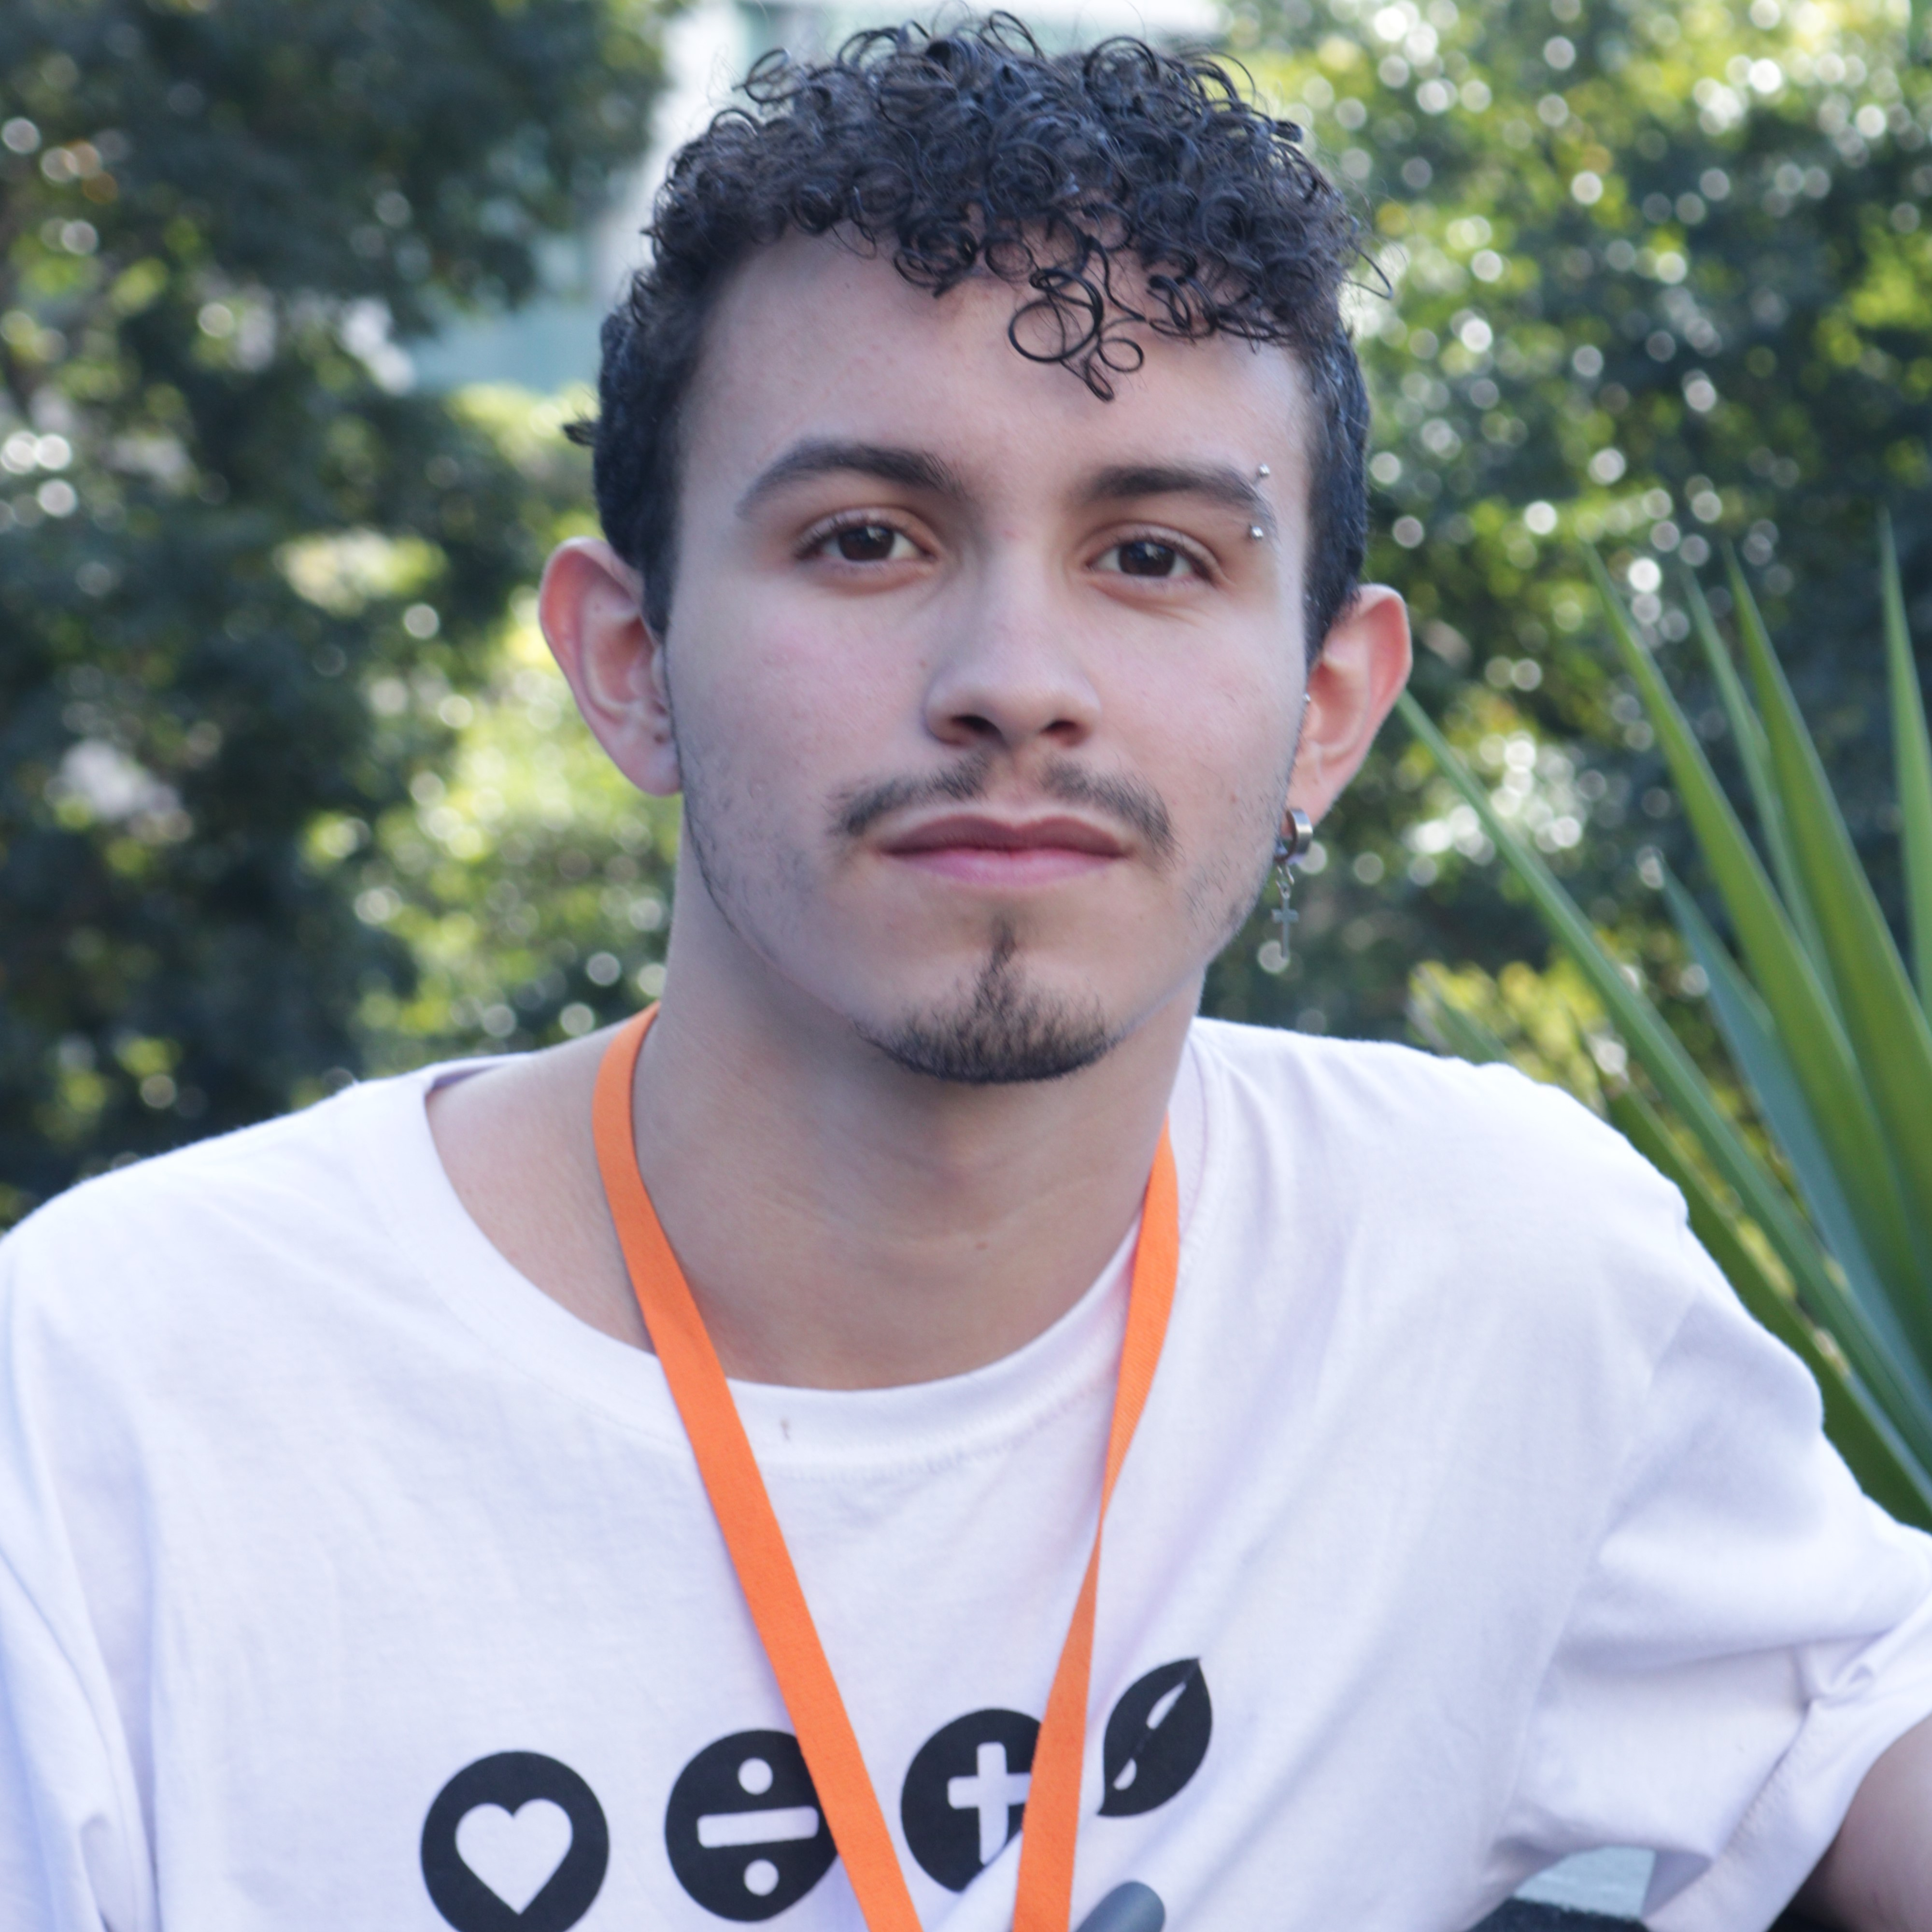
\includegraphics[scale=0.25, width= 40mm]{foto3.jpg} % Picture
        \end{minipage} \hfill
        \begin{minipage}{0.65\textwidth} % Name and Contact Info
            \name{Leonardo Porto}{Mestrando de Astronomia} % Name and Profession
            \vspace{2em}
            \email{leonardo22@ov.ufrj.br} $\cdot$
            \phone{+55 (61) 981053235} \par \vspace{0.5em}
            \address{Rio de Janeiro (RJ)} $\cdot$
            \github{https://github.com/}{slowporto}
        \end{minipage}
        
    \end{tcolorbox}

    %%% Sections %%%
    \vspace*{-1em}
    \tcbset{colframe=white,colback=white,arc=0mm, height=0.8\textheight}
    \begin{tcolorbox}
        \vspace*{-0.5em}
        \begin{minipage}[t]{0.3\textwidth} % Side Panel (e.g. Skills, Links, Languages, etc.)
            \begin{tcolorbox}[height=0.8\textheight, grow to left by=0.6cm,colback=backdrop,colframe=backdrop,arc=0mm]

                % Skills, the skill level is drawn as bars, input: skill name and an array starting from 0 and ending before 4
                \subsection*{Habilidades}
                    \skill{Python}{0, 1, 2, 3, 4}
                    \skill{Git}{0, 1, 2, 3}
                    \skill{Linux}{0, 1, 2, 3, 4}
                    \skill{R}{0, 1, 2, 3}
                    \skill{LaTeX}{0, 1, 2, 3}

                \subsection*{Línguas}
                    \lan{Português}{0, 1, 2, 3, 4}
                    \lan{Inglês}{0, 1, 2, 3, 4}
                    \lan{Espanhol}{0, 1, 2, 3, 4}
		    \lan{Alemão}{0, 1, 2}
            \end{tcolorbox}
        \end{minipage}
        \begin{minipage}[t]{0.7\textwidth} % Main Panel (e.g. Education, Work Experience)
            \begin{tcolorbox}[grow to right by=0.75cm,height=0.8\textheight,colframe=white,colback=white]

                % Profile Section
                \section*{Perfil Profissional}
                    Graduado em astronomia pelo Observatório do Valongo (UFRJ), mestrando em Astronomia pelo IAG-USP. 

                % Education
                \section*{Formação Acadêmica}
                    \education{Bacharelado - Astronomia}{Abril 2022 - Dez 2025}{Universidade Federal do Rio de Janeiro}{Graduação em Astronomia pelo Observatório do Valongo da UFRJ.}
		    \education{Mestrado - Astronomia}{2026 - (atual)}{USP}{Mestrado em Astronomia pelo IAG - USP}

                % Work Experience
                \section*{Experiências}
                    \work{Jovem Aprendiz (Administrativo)}{Set 2021 - Abril 2022}{SESC DF - Serviço Social do Comércio}{Experiência em serviços administrativos, arquivamento de documentos, lançamento de atestados e atendimento ao público.}  \vspace{2em}
                    \work{Iniciação Científica}{Out 2022 - 2025}{Observatório do Valongo - UFRJ}{Pesquisa de Iniciação Científica na área de evolução química da galáxia, trabalhando com tratamento de dados usando Python e R, manuseamento de catálogos e outras ferramentas. } \vspace{2em}
                    \work{Projeto de Extensão}{Set 2022 - Jun 2023}{Observatório do Valongo - UFRJ}{Participante do projeto de extensão "Astronomia para Poetas" do Obervatório do Valongo. Trabalho de divulgação científica, elaboração de textos paras redes sociais, realização de artes e imagens midiáticas, organização da agenda administrativa.} 
            \end{tcolorbox}
        \end{minipage}
    \end{tcolorbox}
    
\end{document}